\clearpage{\pagestyle{empty}\cleardoublepage}

\chapter{Testbench}

\section{Testbench del componente}

Per testare nello specifico il funzionamento della cache e i meccanismi di comunicazione con la ram, sono stati realizzati 3 file:
 
\begin{itemize}
 \item \texttt{Cache_test_ReadAndWrite.vhd}: nel quale si verifica il corretto funzionamento delle scritture, in primo luogo dentro la cache e poi anche della RAM.
 \item \texttt{Cache_test_ReadAndReplacement.vhd}: nel quale si verifica il corretto funzinamento della politica di rimpiazzamento mediante contatori.

 \item \texttt{Cache_test_snoop.vhd}: nel quale si verifica il corretto funzionamento del meccanismo MESI in caso di eventuali snoop.
\end{itemize}

\subsection{Cache_test_ReadAndWrite.vhd}
Questo File ha in comune, come tutti i file di testbench che si vedranno  in questa sezione, la dichiarazione dei componenti, il portmap e la fase di reset iniziale poi si compone di 3 fasi con le quali si verifica il funzionamento delle scritture:

\subsubsection{Fase 1: Letture d' inizializzazione}
Si caricano in Cache 3 blocchi da 32 byte, 2 in modalit� write-back (\texttt{ch_wtwb='0'}\\) e uno in modalit� write-throght (\texttt{ch_wtwb='1'}\\). occupando rispettivamente la via [0] del primo(di indice [0]), secondo(di indice [1]) e terzo(di indice [2]) set. In particolare nel terzo set si nota come l'attivazione del segnale \texttt{ch_wtwb}\\, porti lo stato del terzo blocco a 1 ovvero a MESI_S, mentre nei altri due casi \`e uguale a "10" ovvero MESI_E.
\begin{figure}[h!]
\centering
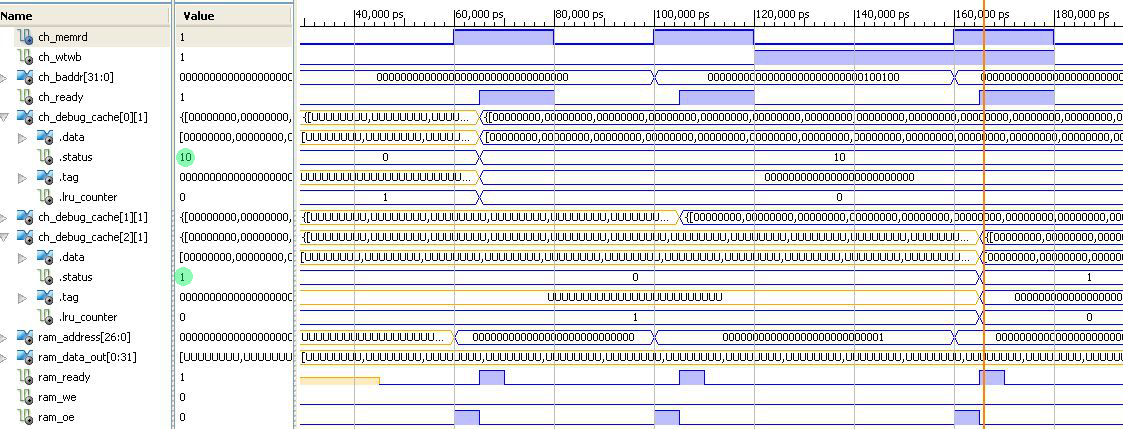
\includegraphics[width=\textwidth]{img/testbench/ReadAndWriteFase1.JPG}
\caption{screenshot ISIM fase 1}
\label{fig:write1}
\end{figure}

\subsubsection{Fase 2: Scritture}
Nella prima scrittura (evidenziata in verde nell'immagine) avviene un miss in quanto il blocco di TAG=*10 non � ancora presente in cache, verr� quindi effettuata prima una lettura in RAM per leggere il blocco contenente il dato e portarlo nella seconda([0]) via del primo set , aggiornati i valori dei contatori che gestiscono l'invecchiamento per il meccanismo di rimpiazzamento,e quindi effettuata una scrittura in cache aggiornando il valore della word di offset "00110" (ovvero il byte dalla posizione [6] alla [9]), e lo stato della via viene posto a MESI_M ("11").
Nella seconda scrittura avviene una scrittura su di un gi� blocco presente in cache, quindi si modifica semplicemente il dato e si aggiorna lo stato come nel caso precedente.
Nella terza scrittura  (evidenziata in azzurro nell'immagine) invece a differenza dei due casi precedenti, la via e in modalita write-throught e non write-back di conseguenza, la scrittura oltre ad avvenire in cache, avviene anche in RAM, ed essendo il nostro caso a monoprocessore la anzich� porsi in stato MESI_M, come negli altri casi si pone in MESI_E in quanto il contenuto del blocco in cache � uguale a quello a ci� che c'\`e al livello superiore (nel nostro caso la RAM).

\begin{figure}[h!]
\centering
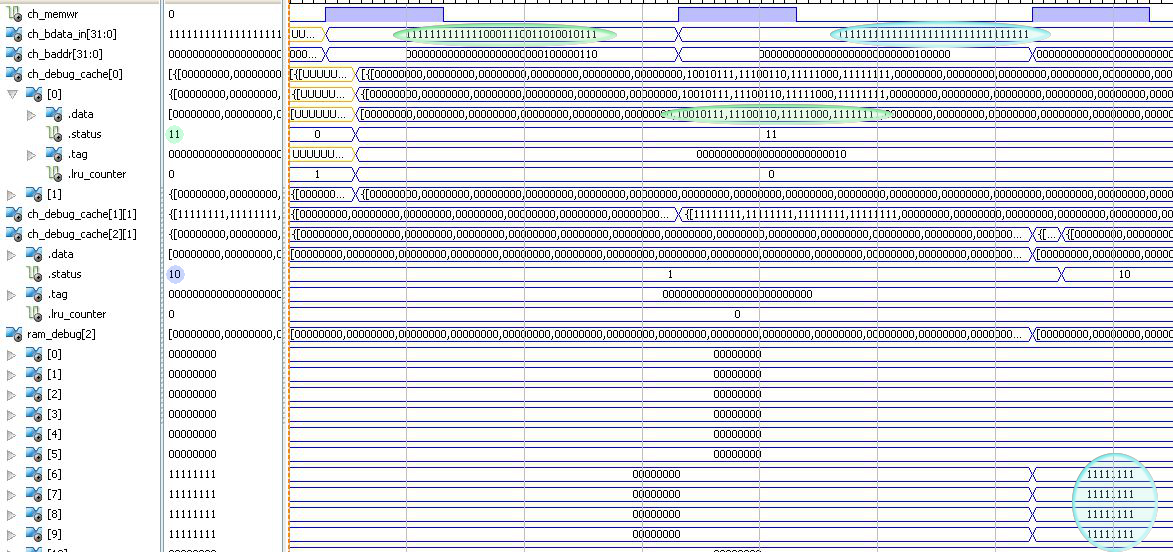
\includegraphics[width=\textwidth]{img/testbench/ReadAndWriteFase2.JPG}
\caption{screenshot ISIM fase 2}
\label{fig:write2}
\end{figure}

\subsubsection{Fase 3: Letture di verifica}
In questa ultima fase vengono fatte delle letture; nel primo caso due letture per verifare i dati scritti nelle prime due scritture.
Nel secondo caso(riportato in figura) si obbliga la cache ad effetture un replacement, in modo da vericare che la cache esegua correttamente il salvataggio in RAM e poi viene ricaricato il blocco originariamente modificato, e si nota che effettivamente il dato che ci viene restituito � quello che era stato originariamente scritto in cache.

\begin{figure}[h!]
\centering
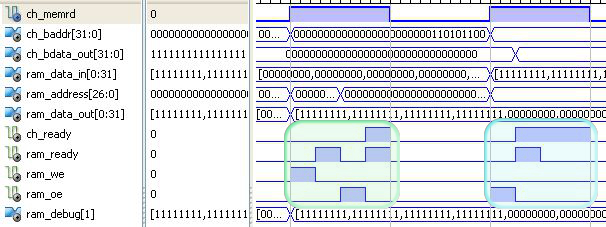
\includegraphics[width=\textwidth]{img/testbench/ReadAndWriteFase3.JPG}
\caption{screenshot ISIM fase 3}
\label{fig:write3}
\end{figure}

Nella figura\ref{fig:write3} si nota inoltre la sequenza di segnali che vengono utilizzati fra RAM e CACHE per comunicare in particolare, all'attivazione del segnale ch_memrd nel primo caso per scrivere un blocco modificato presente in CACHE da rimpiazzare con un nuovo blocco(in verde) e nel secondo caso per una lettura in RAM per portare un dato in CACHE (in azzurro).

\subsection{Cache_test_ReadAndReplacement.vhd}

Questo file ha in comune, come tutti i file di testbench che si vedranno in questa sezione, la dichiarazione dei componenti, il portmap e la fase di reset iniziale poi si compone di 3 fasi con le quali si verifica il corretto funzionamento del meccanismo dei contatori per la politica di rimpiazzamento, durante una serie di letture e si analizzera anche il caso in cui la CACHE subisca un invalidazione di una linea.

\subsubsection{Fase 1: Letture d' inizializzazione}
Nella prima fase si effettuano 8 letture per riempire tutta la CACHE, quindi si avr� che tutti i contatori nelle vie, dei quattro set, che sn stati utilizzati per ultimi con il contatore a "0" metre le altre vie saranno a "1".

\subsubsection{Fase 2: Invalidazione}
Nella seconda fase verra eseguita un invalidazione sul blocco di TAG="*010" che con index="10", ovvero il terzo set; questo comporta il portare lo stato da MESI_E(10) a MESI_I(0) e contatore a "1" nella via che lo contiene mentre l'altra via del set sar� portatata a "0".

\subsubsection{Fase 3: Verifica meccanismo contatori}

Con la prima lettura si verifica che se si effetua una lettura di una word contenuto in un blocco(di TAG="0") presente in CACHE (hit)  il contatore della via dove � contenuto viene quindi resettato, mentre le altre vie con valore pi� basso vengono incrementate.

Con la seconda lettura si richiede un dato contenuto in blocco non presente in cache (miss), viene quindi selezionato il set in base al valore dell' indice, "01" in questo caso e verr� rimpiazzato il blocco con valore del contatore pi� elevato che in questo caso corrisponde alla via con TAG="10" (la via [0]) nella quale si era precedentemente resettatato il contatore della via [1], senza effettuare nessuna scrittura in RAM in quanto il blocco � in stato MESI_E.

Con la terza lettura invece si richiede un dato contenuto in un blocco non presente in cache e con indice="10" , che corrisponde al terzo set sulla quale via precedentemente era stata eseguita un invalidazione, via che verra quindi rimpiazzata con il blocco con TAG="110".

\begin{figure}[h!]
\centering
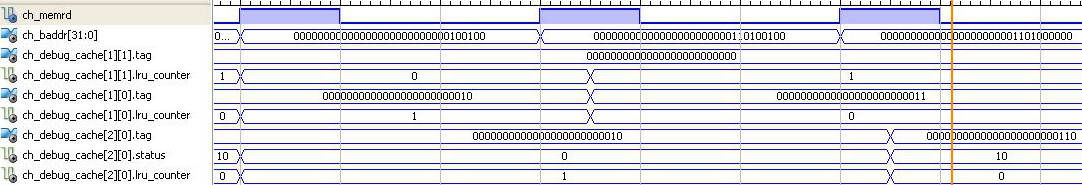
\includegraphics[width=\textwidth]{img/testbench/ReadAndReplacementFase3.JPG}
\caption{screenshot ISIM 3 letture}
\label{fig:replacement3}
\end{figure}

Inifine vengono eseguite una serie di letture su blocchi presenti e non su diversi set, per verificare che tutto nel complesso funzioni correttamente.

\subsection{Cache_test_snoop.vhd}
Questo file ha sempre in comune, come tutti i file di testbench che si sono visti in questa sezione, la dichiarazione dei componenti, il portmap e la fase di reset.

Quindi si procede con l'inizializzazione della cache per verificare il corretto funzionamento dello snoop. Nello specifico si porta in cache due blocchi dalla RAM e del secondo ci si esegue una scrittura per portarlo in stato MESI_M.

In secondo luogo si procede con l'attivazione del segnale di snoop ovvero:\texttt{ch\_eads}\\ e impostato l'indirizzo su cui fare lo snoop:\texttt{ch\_snoop\_addr}\\. La CACHE risponder� in modo opportuno i segnali di \texttt{ch\_hit,ch\_hitm}\\ e modificando eventualmente lo stato delle vie.

Nel primo caso si effettua uno snoop su di un blocco che non \`e contenuto in cache, quindi la cache risponder� con  \texttt{ch\_hit="0",ch\_hitm="0"}\\.

Nel secondo caso(evidenziato in giallo in Fig.\ref{fig:snoop1}) si effettua uno snoop su di un blocco presente in cache in stato MESI_E, quindi la cache risponder� con \texttt{ch\_hit="1",ch\_hitm="0"}\\ e porter� lo stato della via in MESI_S("1").

Nel terzo caso(evidenziato in verde in Fig.\ref{fig:snoop1}) si effetuer\`a uno snoop su di un blocco che \`e presente in cache in stato MESI_M("11"), la cache risponder� quindi:  
\begin{itemize}
\item \texttt{}\texttt{portando ch\_hit="1" e ch\_hitm="1"}\\
\item \texttt{}\texttt{effettuando la scrittura in RAM del blocco contenuto in cache.}\\
\item \texttt{}\texttt{portando lo stato della via in MESI_S("1")}\\
\end{itemize}
\begin{figure}[h!]
\centering
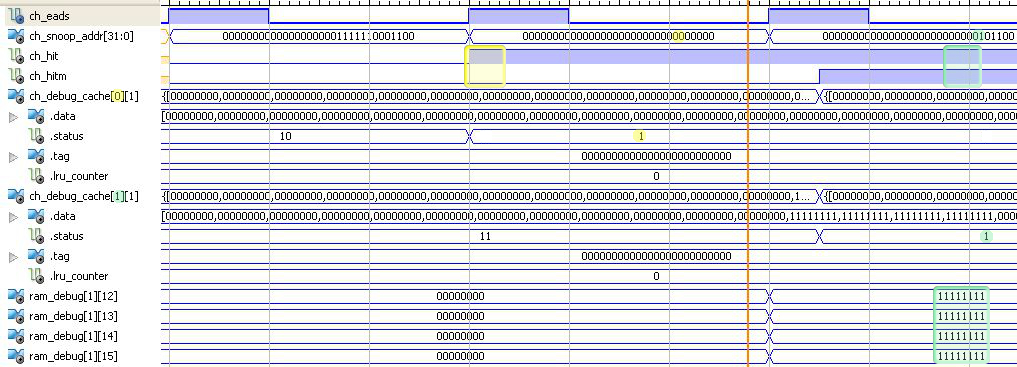
\includegraphics[width=\textwidth]{img/testbench/Snoop1.JPG}
\caption{screenshot ISIM 3 casi di snoop}
\label{fig:snoop1}
\end{figure}
Infine si effettua una scrittura sul blocco precedentetemente portato in MESI_S,
per verificare che la CACHE scrivi effetivamente i dati in RAM.

\section{Assembler per DLX}

Dopo avere testato individualmente il funzionamento dei componenti CACHE e della RAM, si \`e passati al test del corretto funzionamento della cache inserita all'interno del progetto del processore DLX.\\
Per far ci\`o sono stati realizzati una serie di programmi in assembler, della quale mostreremo solo i due maggiormente significativi:
\begin{itemize}
 \item \texttt{provaReplacement123}: nel quale si verifica la corretta comunicazione tra cache e DLX e il meccanismo di rimpiazzamento.
 \item \texttt{provaFU}: nel quale si verifica il corretto funzionamento della Forwarding unit. 
\end{itemize}

\subsection{Dal codice all'escuzione}
Per completezza in questa sezione si spiegher\`a brevemente come poter mettere in esecuzione un codice assembler.
In primo luogo \`e necessario scrivere il codice in assembler all'interno di un file con estensione *.dls, che viene poi dato in pasto all'assemblatore DASM. Quest'ultimo lo converte in codice macchina mediante il seguente comando, eseguito dal prompt di comandi Windows:\\

\texttt{dasm -a -l <nome\_file>.dls}\\

Il risultato sar\`a un file \texttt{<nome\_file>.dlx} che a sua volta dovr\`a essere convertito mediante la classe java \texttt{DLXConv},eseguendo dal prompt di comandi Windows:

\texttt{java DLXConv <nome\_file>.dlx}\\

 per avere un file  \texttt{<nome\_file>.dlx.txt} contenente il codice in un formato direttamente inseribile all'interno del progetto del DLX.\\

In particolare quest'ultimo dovr\`a essere inserito nel file \texttt{Fetch\_Stage.vhd} all'interno dell'array che sostituisce la EPROM contenente le istruzioni in linguaggio macchina, da dare in pasto al processore:\\

\lstset{language=VHDL, caption=Inserimento del codice nella memoria istruzioni, label=DescriptiveLabel, breaklines=true, basicstyle=\small, showspaces=false, showtabs=false, stringstyle=\ttfamily, showstringspaces=false,  tabsize=3} % basicstyle=\tiny\ttfamily}

\begin{lstlisting}

constant EPROM_inst: eprom_type(0 to 11) := ( 
-- istruzioni in linguaggio macchina.
);

\end{lstlisting} 

\subsection{Codice assembler}
In questo paragrafo si analizzeranno nel dettaglio i codici assembler dei due test pi\`u significativi.
Per comodit\`a si riporter\`a il codice contenuto nella \texttt{EPROM\_inst} corredato di commento e codice assembler relativo.

 \subsubsection{provaReplacement123}
\lstset{language={[x86masm]Assembler}, caption=Codice assembler per il test del meccanismo di rimpiazzamento, label=DescriptiveLabel, breaklines=true, basicstyle=\footnotesize\ttfamily, showspaces=false, showtabs=false, showstringspaces=false,  tabsize=3} % basicstyle=\tiny\ttfamily}

\begin{lstlisting}
X"20010000",	--l1: addi r1,r0,0 ; azzera r1
X"20020001",	--l2: addi r2,r0,1 ; imposta a 1 r2
X"AC220000",	--l3: sw 0(r1),r2 ; memorizzza il valore di r2 all'indirizzo 0+r1(via 1 dell index0)
X"20420001",	--l4: addi r2,r2,1 ; incrementa r2
X"AC220100",	--l5: sw 16#100(r1),r2 ; memorizzza il valore di r2 all'indirizzo 16#100+r1(via 0 dell index0)
X"20420001",	--l6: addi r2,r2,1 ; incrementa r2
X"AC220080",	--l7: sw 16#80(r1),r2 ; memorizzza il valore di r2 all'indirizzo 16#80+r1(replacement via 1 dell index0) 
X"8C220000",	--l8: lw r2,0(r1) ; ripristina valore iniziale di r2 (1)
X"20210004",	--l9: addi r1,r1,4 ; incremento di 4 indirizzo di base in r1
X"0BFFFFE0",	--l10: j l3 ;
X"FFFFFFFF",	--NOP 
X"FFFFFFFF" 	--NOP

\end{lstlisting} 
A lato pratico questo codice conta fino a tre (da qui il nome del file termina con 123), e ad ogni iterazione ricomincia da uno, soltanto che ogni risultato intermedio viene salvato in memoria in una locazione diversa in modo da obbligare la cache ad ogni iterazione di rimpiazzare un blocco sempre lavorando nel primo set, infatti ad esempio nella prima iterazione quando r1="0",si nota che i due bit che identificano l'indice sono sempre uguali a "00".

l3-> 0(r1)=0+0= "000 00 00000"->prima([1]) via occupata nel primo set
l5-> 16#100(r1)="010 00 00000"->seconda([0]) via occupata nel primo set
l7-> 16#80(r1)= "001 00 00000"->prima([1]) via rimpiazzata nel primo set, quindi si ha una scrittura in RAM del blocco modificato e caricamento del nuovo blocco.

A questo punto si effettua il caricamento in r2 del primo valore (ovvero "1"), ma il blocco che contiene la word di indirizzo 0 non \`e pi\`u presente in cache, verra quindi effettuato un ulteriore rimpiazzamento per� sulla seconda via([0]). infine si incrementa in valore di r1 di quattro unita in modo da scrivere non pi\`u nella word di offset "00000" ma di "00010", ovvero la word successiva di ogni blocco.

\begin{figure}[h!]
\centering
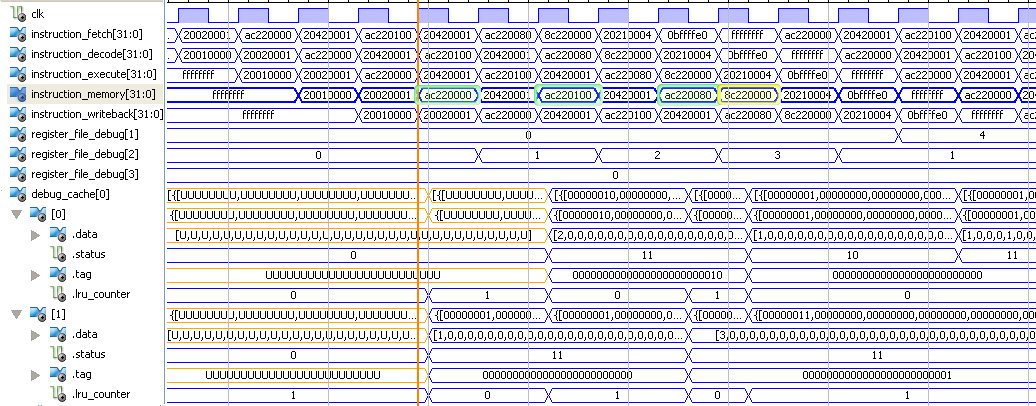
\includegraphics[width=\textwidth]{img/testbench/DLX123.JPG}
\caption{evidenziato in verde le store e in giallo le load}
\label{fig:DLX123}
\end{figure}

\subsubsection{provaFU}

\lstset{language={[x86masm]Assembler}, caption=Codice assembler per il test della Forwarding Unit, label=DescriptiveLabel, breaklines=true, basicstyle=\footnotesize\ttfamily, showspaces=false, showtabs=false, showstringspaces=false,  tabsize=3} % basicstyle=\tiny\ttfamily}

\begin{lstlisting}
X"20420001",  --l1: addi r2,r2,1  ; porta a 1 il valore di r2
X"AC220000",  --l2: sw 0(r1),r2  ; salva il contenuto di r2
X"8C230000",  --l3: lw r3,0(r1)  ; porta in r3 il valore presente in r2
X"20620001",  --l4: addi r2,r3,1  ; incrementa r2
X"0BFFFFF0",  --l5: j l2          ; salta a l1
X"FFFFFFFF",  --NOP

\end{lstlisting} 

In questo programma si testa il corretto funzionamento della Forwarding Unit, infatti nel quinto ciclo di clock si nota che l'istruzione(X"20620001") nello stadio di EX vuole leggere il valore contenuto in r3 per incrementarlo di uno ma \`e appena stato caricato dalla CACHE nell'istruzione presente nello stadio di MEM, quindi la Forwarding Unit fornir� il dato presente nello stadio di MEM attraverso i segnali mem\_dest\_register e mem\_dest\_register\_data allo stadio di EXE.

\begin{figure}[h!]
\centering
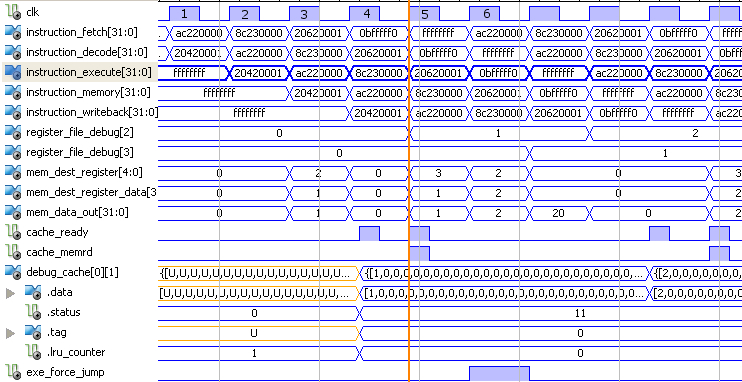
\includegraphics[width=\textwidth]{img/testbench/DLXFU.JPG}
\caption{evidenziato l'istruzione che senza FU porterebbe a degli stalli}
\label{fig:DLXFU}
\end{figure}
